\documentclass{udpreport}
\title{Ruteo Estático y Dinámico}
\author{Integrantes: Francisca Carrrasco, Ignacio López, Nicolás Ramírez.\\Profesor: José Pérez
\\Ayudante: Alexis Inzunza}
\date{Mayo de 2017}
\usepackage{graphicx}
\graphicspath{ {Imagenes/} }
\udpschool{Escuela de Informática y Telecomunicaciones}

\begin{document}
\maketitle
\tableofcontents
\listoffigures
\chapter{Actividades}
	\section{Topología base}
	Lo primero que hicimos fue poner cuatro routers, cuatro switches y dos computadores por cada uno de estos.
	 A continuación se pocisionaron los dipositivos en el espacio de manera que los nombres de las interfaces y de los cables se puedan leer. Luego se conectaron los ordenadores a los switches y estos a los
	routers, hecho esto se procede a instalar el módulo serial en los routers(los cuales se apagaron primero) e inmediatamente se les inserto el módulo. Hecho lo anterior se procedió a interconectar los router entre sí, esto se realiza  a través de un cable serial, una vez terminado esto se prosigue con los comandos y conexiones siguientes\\
	\begin{figure}[h]
	\centering
	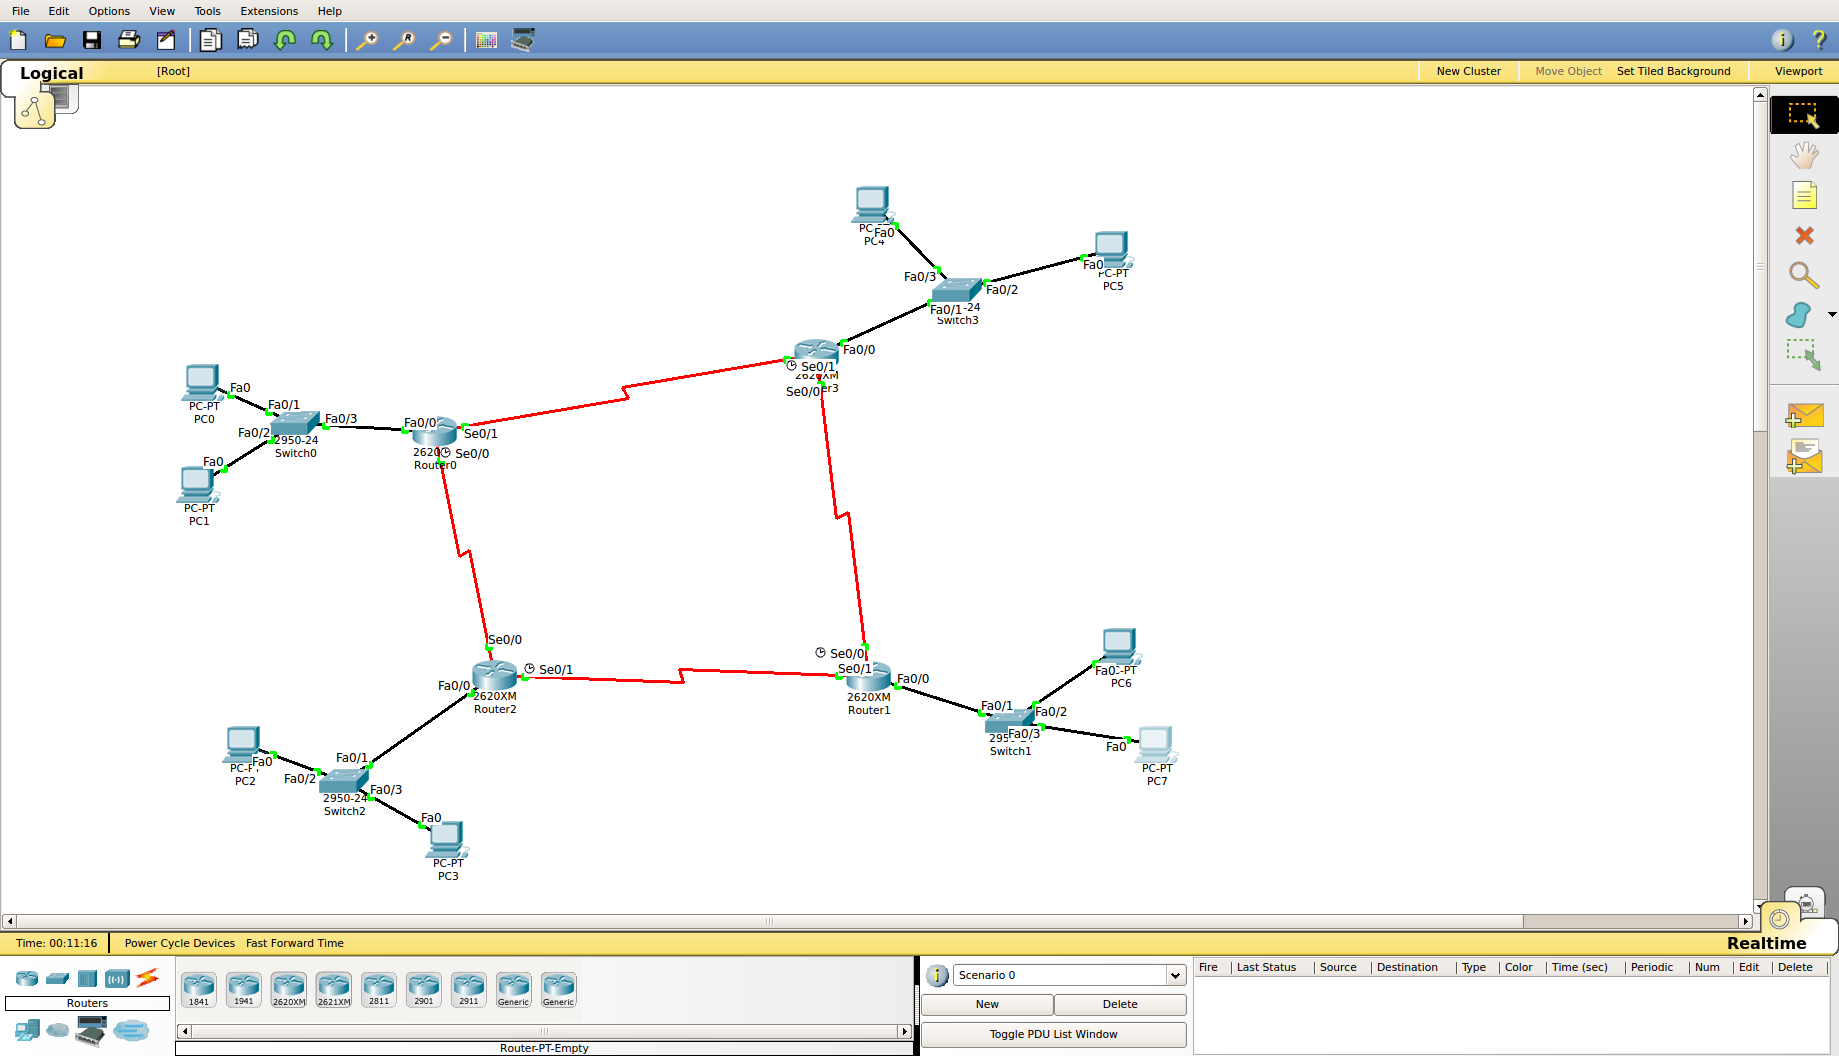
\includegraphics[width=16cm, height=11cm]{Topologia_Base.png}
	\caption{Construcción de la Topología Base}
	\end{figure}
	\newpage
	\section{Configuración Equipos}
	Se configuran los equipos de manera que cada grupo de PC pertenezca a una subred distinta, esto se hace en las configuraciones de cada PC donde se le asignan IPs y gateway manualmente, y luego se configura el router asignándole a la interfaz una IP perteneciente a la subred común con los PC. También se configuran las interfaces de los enlaces seriales de cada router con una subred distinta para establecer un canal comunicación entre ellos.
	\begin{figure}[h]
	\centering
	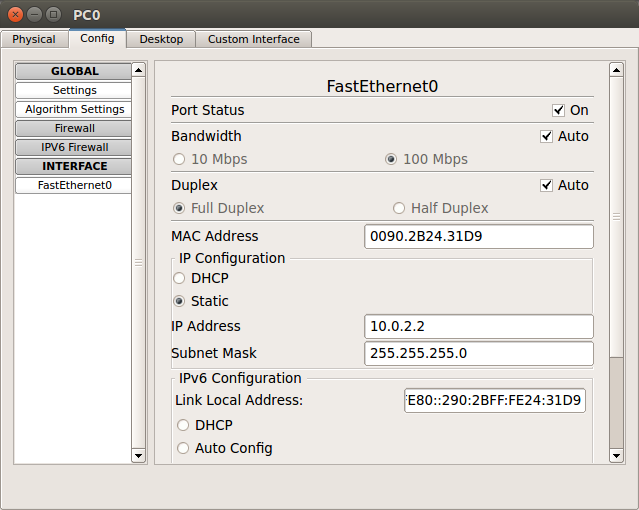
\includegraphics[width=8cm, height=7.6cm]{PC0.png}
	\caption{Configuración de los equipos}
	\end{figure}
	\newpage
	\section{Configuración ruteo estático}
	Se ingresa a la terminal del router, luego indicándoles la IP de destino, porque puerto sale, y la IP por donde da el salto para llegar a destino, esto se debe hacer con cada interfaz del router, de manera que dirija cada paquete que reciba a una interfaz y lo pueda enviar. Lo anterior descrito se debe hacer con cada router.//
	\begin{figure}[h]
	\centering
	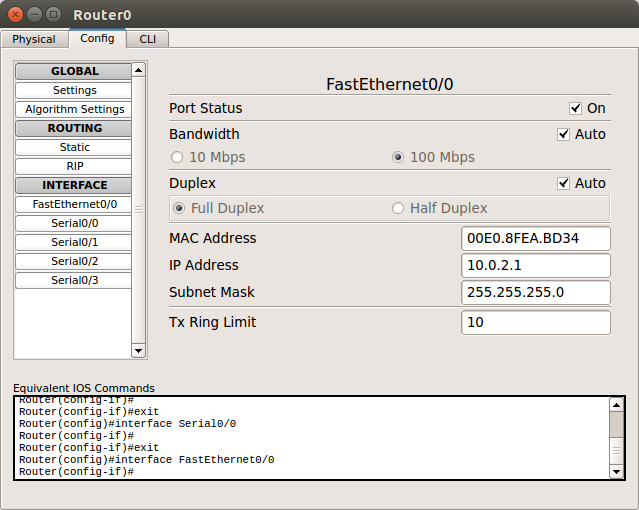
\includegraphics[width=8cm, height=7.6cm]{Router0.png}
	\caption{Configuración de ruteo estático en el router R0}
	\end{figure}
	\newpage
	\section{Configuración ruteo dinámico}
	Se ingresa a la terminal del router y se activa RIP V2 de esta manera se configura automáticamente y sólo tenemos que
	indicarle al router cuál es la red que va a utilizar. Esto se logra al ingresar los comandos que estaban especificados en la guía.
	\begin{figure}[h]
	\centering
	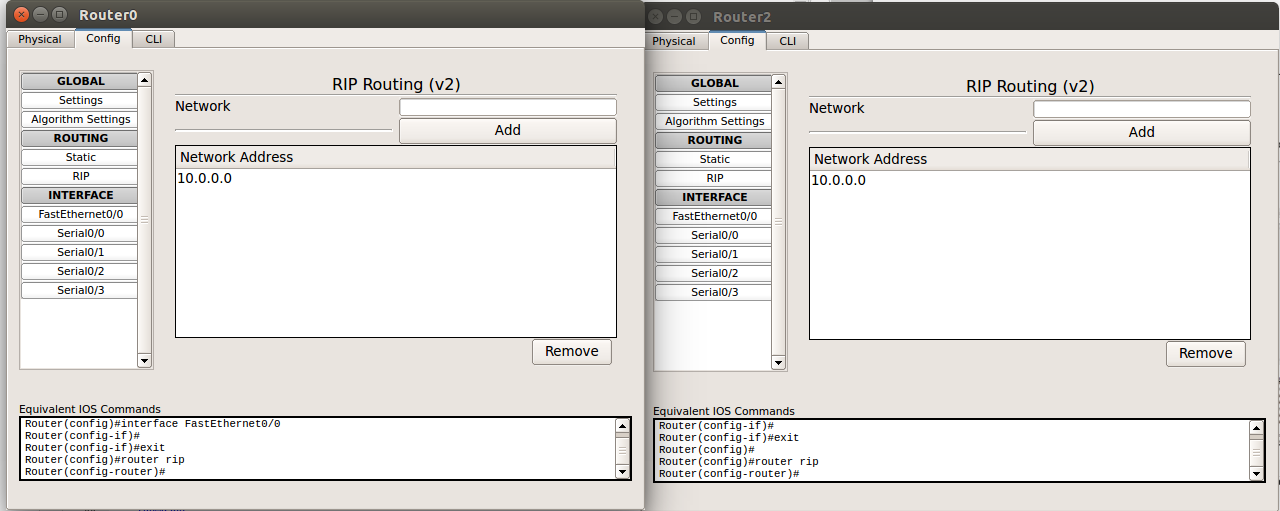
\includegraphics[width=18cm, height=10cm]{rip1.png}
	\caption{Configuración de ruteo dinámico en los router R0 y R2}
	\end{figure}
	\newpage

	
\chapter{Conclusión}
 Al finalizar esta experiencia se ha podido comprobar que el ruteo estático es útil en redes simples, ya que se debe configurar manualmente. En cambio, el ruteo dinámico es útil en redes complejas, ya que se configura de forma automática. Además, se ha aprendido a configurar ruteos dinámicos con el protocolo RIP V2.\\
 
\begin{thebibliography}{x}
\bibitem{Cisco} \textsc{Cisco },
\textit{cisco.utmetropolitana.edu.mx}

\end{thebibliography}

\end{document}
